\section{Measured computational results}\label{sec:results}
\subsection{One full $S$-grid, with or without reusable inverse mapping}
The principal case now uses $n=48,d=3,\mu=0,R=1$, the SVD backend and five selection criteria. Both policies evaluate \emph{exactly the same 17 normalized-smoothness candidates}, including $S=0$ and $S=1$: native-$S$ repeatedly invokes $\Lambda_{n,d}$, whereas the cached policy translates the grid once and reuses its penalties. This is an equal-estimator computational comparison, not a contest between different statistical grids. The recorded two-seed median timing values are inserted automatically from the original Windows CSV, not manually estimated. Although the candidate grid includes $S=0$ and $S=1$, some criterion values at those endpoints can be mathematically undefined (notably residual BIC at interpolation), and those scores are not reinterpreted as admissible optima.

% AUTO-GENERATED FROM ARCHIVED WINDOWS DATA; DO NOT EDIT
\begin{table*}[t]
\caption{Five completed 17-point selection searches for $d=3$, $n=48$, fixed $\mu=0$, SVD, $R=1$. Values are two-seed medians in milliseconds. Both policies evaluate the identical full $S\in[0,1]$ grid; premapped standalone time includes conversion once per criterion.}
\label{tab:criteria}\centering
\begin{tabular}{lrr}
\toprule
Criterion & Repeated $S$ inversion & Premapped $S$ grid \\
\midrule
CV & 2.058 & 1.846 \\
GCV & 1.958 & 1.723 \\
AICc & 2.024 & 1.724 \\
Residual BIC & 1.972 & 1.724 \\
Profiled Gaussian ML & 2.038 & 1.776 \\
\bottomrule
\end{tabular}
\end{table*}


\begin{figure*}[t]\centering
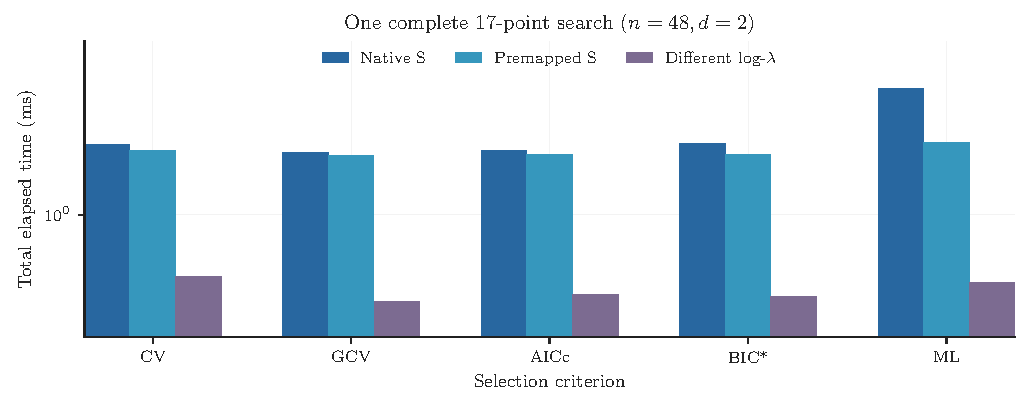
\includegraphics[width=\textwidth]{figures/criterion_coordinates.pdf}
\caption{Full $S\in[0,1]$ selection at $d=3$, $n=48$, fixed $\mu=0$ and SVD, with five criteria: repeated on-demand $S\mapsto\lambda$ inversion versus one cached candidate translation. Both policies evaluate identical penalties. Bars are observed two-seed median standalone timing results, including one-time mapping cost in the second policy.}
\label{fig:coordinates}
\end{figure*}

For a second, historically reported $d=2$ comparison at the same $n=48,\mu=0,R=1$, the archived five native-$S$ searches total 11.234\,ms, versus 3.980\,ms when the grid is mapped once and shared across five backend-only searches: a descriptive factor of 2.823. These $d=2$ values are \emph{not} relabeled as $d=3$ timings; the new $d=3$ table and plot use their own archived records. Within each difference order, a precomputed grid can be shared across criteria, series and fixed $\mu$ values without altering the PLS estimator.

\subsection{One evaluation, full grid and repeated independent series}
Figure~\ref{fig:workloads} plots all seven backends at a \emph{single} $s=0.5$ GCV score, one mapped 17-point GCV grid and eight independent full-grid GCV searches, under fixed $n=48,d=3,\mu=0$. It uses the original full-factorial Windows rows, drawing a timing only where both experimental seeds completed that particular workload with valid numerical scores. Unsuccessful or incomplete cases are missing, not assigned fictitious times. The figure makes visible why a one-evaluation ranking need not generalize to selection or reuse workloads: decomposition cost is paid once, while data projections, curve solves and per-candidate trace work scale differently across algorithms.

\begin{figure*}[t]\centering
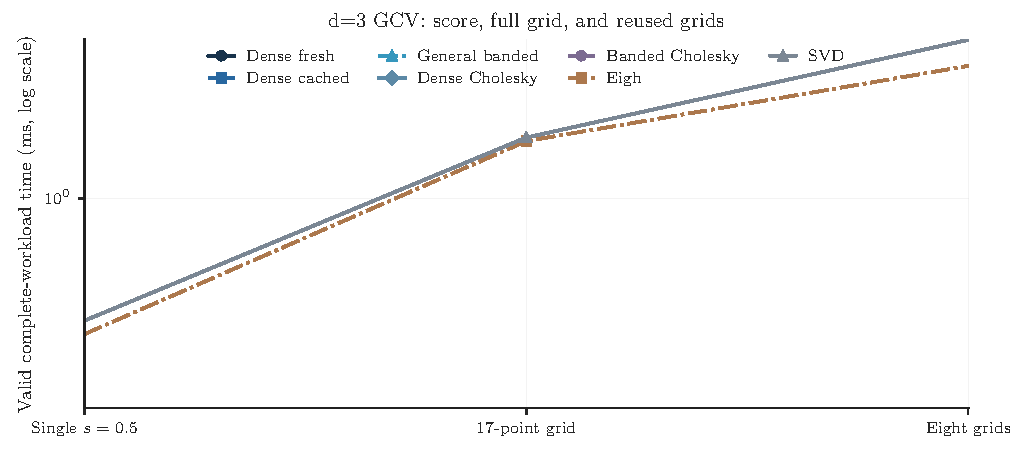
\includegraphics[width=\textwidth]{figures/workload_scaling.pdf}
\caption{Observed standalone elapsed time for one GCV score ($s=0.5$), one 17-point grid, and eight independent grids, across seven implementations. Data are from the two-seed Windows full factorial with $n=48,d=3,\mu=0$ and shared preparation. Points are shown only for workloads with complete numerically valid seed pairs; missing points correspond to unvalidated/unsuccessful computations, not zero elapsed time. The three workload classes are distinct algorithms, not repeated scalar multiplications of one measured time.}
\label{fig:workloads}
\end{figure*}

\subsection{Repeated grid reuse and difference order}
Figure~\ref{fig:reuse} shows the recorded ratio of cold to shared backend-only time for $R=8$ complete $s$-grid searches across $d=1,\ldots,5$, conditional $\mu=0$, $n=48$, and the SVD backend. Differences among criteria are attributable to distinct scoring operations and reuse boundaries, not a change in statistical PLS formulation. A ratio greater than one favors shared setup for that cell; outcomes missing the necessary two valid seeds are left blank, not silently imputed.

\begin{figure*}[t]\centering
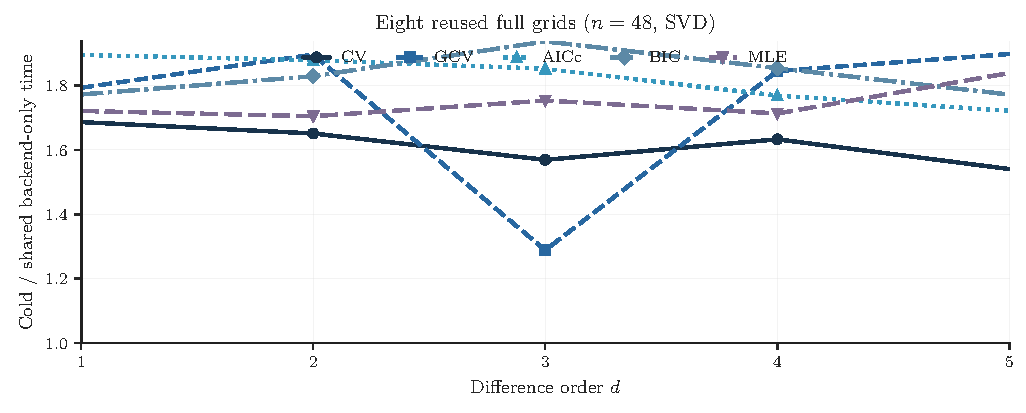
\includegraphics[width=\textwidth]{figures/reuse_by_d.pdf}
\caption{Cold versus shared implementation cost for eight repeated matched-grid selections by difference order and criterion. A vertical value above one indicates less backend-only time with shared preparation. $n=48$, fixed $\mu=0$, SVD; exact source is the archived two-seed Windows timing CSV. No $d=6$ Windows timing was recorded.}
\label{fig:reuse}
\end{figure*}

\subsection{Longer series and repeated fitted curves}
The separate complete-trend benchmark, with $n$ extending to 400 and up to 256 repeated fits, documents substantial changes in winners. For $n=400,d=2,\mu=0$, the ratio of fresh dense to spectral total time was 0.158 at $M=1$ but 28.314 at $M=256$; 0.158 means the dense approach was faster for the single fit, whereas 28.314 means the spectral implementation was faster than the repeatedly fresh dense solver on the larger sweep. Against a properly general banded solver the corresponding ratios were 0.055 and 0.339, so \emph{banded remained faster} in those two recorded workloads. These are host-specific paired cases, not universal crossovers and not five-criterion selections.

The independent 20-seed solver study also supports comparing higher orders. Figure~\ref{fig:solver} shows the original paired geometric-mean SVD/banded-Cholesky total-runtime ratio at $n=96$, $M=16$ complete fitted curves, fixed $\mu=0$, and orders $d\in\{1,2,3,5\}$. There is \emph{no} paired $d=4$ observation for this exact workload in that source: the figure does not interpolate or fabricate one. A ratio above one favors banded Cholesky and below one SVD. These are \emph{fit-only} timings and do not cover trace, leverage or five-criterion selection.

\begin{figure*}[t]\centering
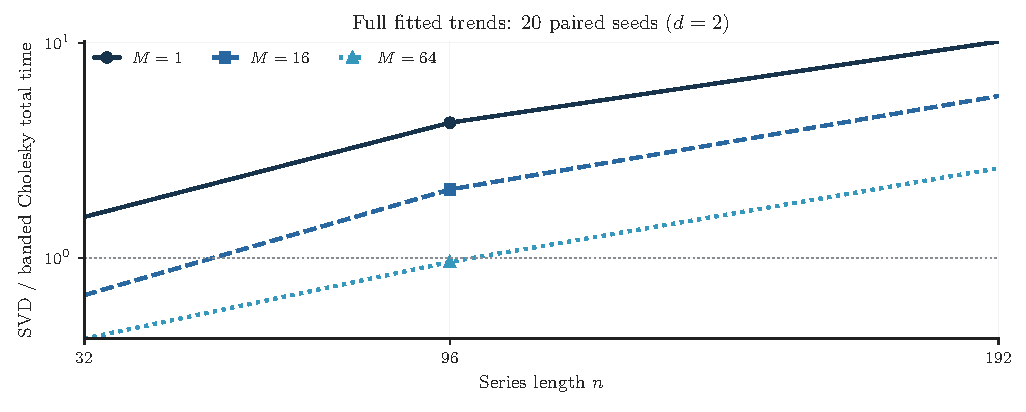
\includegraphics[width=\textwidth]{figures/solver_crossover.pdf}
\caption{Measured paired SVD/banded-Cholesky full-curve total-time ratios across available difference orders at $n=96$, $M=16$ and $\mu=0$. Each order has 20 independent paired data seeds. $d=4$ was not included in this matched solver workload; no result is extrapolated. This is not a criterion-selection benchmark.}
\label{fig:solver}
\end{figure*}

\subsection{Exact matched-grid equivalence}
The complete source audit verified 4,484 numerically valid seed-matched native-$s$/premapped-$\lambda$ grid comparisons with \emph{zero} differences in selected $s$ and scored values. This is expected from \eqref{eq:S}: a monotone coordinate transform does not change the statistical model. The computational advantage lies in \emph{the caching policy}, not statistical changes. Results from unmatched log-$\lambda$ or bounded continuous search cannot establish this equivalence because they evaluate different candidate sets.

No measured cell in this section should be considered an objective benchmark at $d=6$ or for data-derived $\widehat\mu$; those remain future research dimensions.
